\section{Methods}

\subsection{Mechanical model}

The system under investigation is a multi-link inverted pendulum on a cart. This setup, known for its inherent instability and dynamic nature, is a cornerstone in control theory~\cite{Fantoni2001Nonlinear}. The cart, serving as the base platform for the pendulum links, is limited to linear motion along a horizontal track, simplifying the translational dynamics to one-dimensional motion along the x-axis. The cart's movement is controlled by an externally applied force $F$, which is crucial for the system's stabilization. The magnitude and direction of this force significantly impact the system's dynamics, providing a means to counteract the gravitational torque imposed by the pendulum links. The details of the system modelling are described in~\cite{manzl2023relrl}.

\begin{figure}[h]
\centering
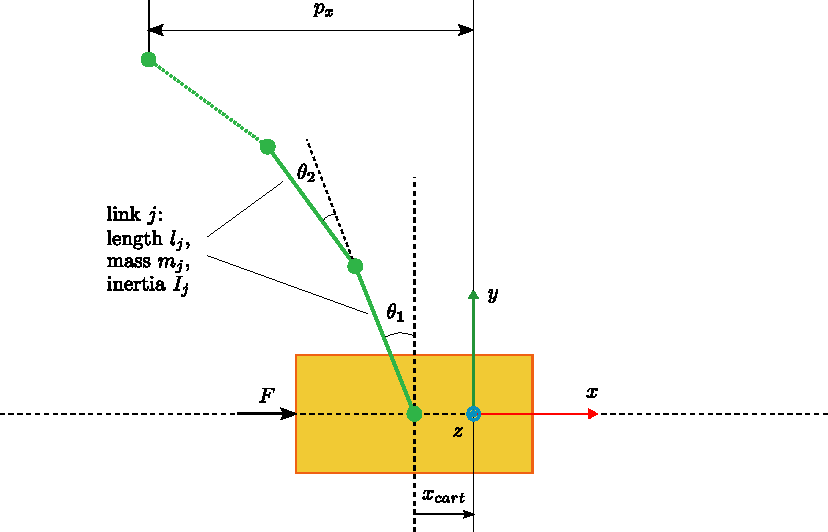
\includegraphics[width=10cm]{Figures/cart_pole_model.pdf}
\caption{$N$-link inverted pendulum on a cart. Minimal coordinates formulation $\mathbf{q} = \mathbf{s} =  [x_{\text{cart}}, \theta_1, \ldots, \theta_N]$ are used to model the system. Each link consists of length $l_j$, mass $m_j$, moment of inertia $I_j$. The cart is a rigid body with mass $m_{cart}$.}
\label{fig: n-pendulum on a cart}
\end{figure}

Attached to the cart is a series of n rigid links, each connected end-to-end by revolute joints. These joints allow for free rotational movement in the vertical plane, and each link 
$j$ is characterized by mass $m_j$, length $l_j$ and inertia $I_j$.
This model, with its high degree of control difficulty and relevance to real-world applications, provides a valuable platform for testing sophisticated control algorithms, including those based on Reinforcement Learning.

\subsection{Reinforcement Learning with continuous action space}
Reinforcement Learning is a branch of machine learning where an agent learns optimal behavior through systematic interaction with a dynamic environment, aiming to maximize cumulative rewards. This learning paradigm is distinct from supervised learning; in RL, the agent is not explicitly instructed which actions to take. Instead, it must explore and discover which actions yield the highest rewards by trial and error, a process often facilitated by a policy—a decision-making function that maps states of the environment to actions to be taken in those states~\cite{sutton_reinforcement_2018}.

In our research, RL is employed to train agents to manage the dynamics of a multi-link inverted pendulum on a cart, a challenging control problem that requires maintaining precise dynamic stability throughout the process. The reward function in RL plays a crucial role as it guides the learning process. For instance, a reward function can be designed to penalize the agent for excessive movement away from a target state or for using too much energy, while rewarding closer approximations of the desired state, such as maintaining the pendulum in an upright position. We use the reward function, which has shown one of the best performances from our previous study
\begin{equation}
r = 1 - w_p \frac{\left|p_x\right|}{\chi_\mathrm{cart}} - (1-w_p) \frac{\sum_{j=1}^\mathrm{N} \left|\theta_j\right|}{\mathrm{N} \chi_{\theta}} 
\label{eq:reward}
\end{equation}
It combines a tip position with the sum of pendulum link angles $\sum_{j=1}^{N} \left|\theta_j\right|$, weighted by a factor $w_p$. $\chi_\mathrm{cart}$ and $\chi_{\theta}$ are predefined, constant position and angle thresholds, which differ from 1-link to more link systems. $\mathrm{N}$ is the number of the links.

In RL, the choice between discrete and continuous action space might significantly affect the performance of learning algorithms. Discrete action space, used in our previous study, limits the agent’s actions to a finite set of possibilities: it either applies a negative or a positive force of the same magnitude to regulate the behavior of the system. In a continuous action space the agent is provided with an interval of the control force
\begin{equation}
F = [-f_\mathrm{cart}, +f_\mathrm{cart}]
\label{eq:force}
\end{equation}
From this interval in Eq.~\eqref{eq:force} the agent is free to choose any suitable control force as an action for learning the stabilization task. Since it provides more possible actions then the discrete action space, it emerges in a faster training of an agent and achieves a more smooth and robust control task execution.  
% NOTE: 1) continue with - adding a final punchline to this section
% While simpler to implement, this can restrict the agent's ability to finely tune its responses to the environment's demands.

\subsection{Model evaluation} \label{Model evaluation}

For the model evaluation we use the same specifications as in our previous research of Manzl et. al.~\cite{manzl2023relrl}. The performance of the agent is periodically evaluated based on the mean reward exceeding a defined threshold \( \lambda_r \) and the loss being below a threshold \( \lambda_l \). During each evaluation, the agent undergoes \( n_{\text{test}} \) tests in an environment simulated for \( n_{\text{eval}} \) time steps, ensuring \( n_{\text{eval}} > n_{\text{learn}} \). For instance, with a time step \( h = 0.02 \) s, \( n_{\text{eval}} = 5000 \) corresponds to a 100 s test duration. During the tests, the agent's initial states are perturbed within a range of \( \pm x_{\text{init}} \), and the maximum norm of the state vector is used to compute the test error \( e_{\text{test},i} = \|\mathbf{s}_i\|_{\infty} \) at each time step \( t_i \). The total test error \( e_{\text{test}} \) is defined as the maximum error encountered in the final quarter of the evaluation period:
\begin{equation}
	e_{\text{test}} = \max(e_{\text{test},i}) \quad \forall \, i \geq \frac{3}{4}n_{\text{eval}}.
\end{equation}
The training is deemed complete when \( e_{\text{test}} \) falls below a pre-determined threshold \( \chi_{\text{test}} \) for all tests, providing a criterion for potential early stopping. To assess model robustness, several agents are trained and evaluated, with their performances depicted as envelopes formed by the best, worst, and mean error metrics across time steps. Notably, early evaluation results (within the first 50,000 steps) may be unreliable due to insufficient model development, necessitating the use of linear interpolation for clearer data interpretation.

\subsection{Performance evaluation of PPO with continuous action space} \label{Performance Evaluation of PPO with Discrete and Continuous Action Spaces}

For the evaluation of an action space benefits in our study we use the PPO RL-algorithm. PPO algorithm itself aims to improve policy gradient methods by optimizing a surrogate objective function while ensuring that updates to the policy do not deviate too far from the previous policy. It accomplishes this by using a clipped objective function that limits the size of policy updates, thereby stabilizing training and improving performance~\cite{schulman2017ppo}. The evaluation is conducted on an N-link inverted pendulum system, specifically analyzing the performance with 1-link, 2-link, and 3-link systems. The analysis explores two different action spaces and their impact on the agent's ability to stabilize the pendulum in the upward-facing equilibrium. 
For all systems, we focus on the task of balancing the inverted pendulum in the unstable upward-facing equilibrium. The challenge increases with the number of links, as each additional link contributes to the overall instability of the system. The single pendulum is a well-known benchmark for RL methods, and this evaluation extends to more complex systems with additional links.
The experiments are conducted using Exudyn Version 1.8.52 and stable-baselines3 Version 1.8.0. Each experiment is repeated 10 times with different random seeds to account for variations in initialization. The PPO algorithm is implemented with standard parameters, except where adjustments are made for the specific requirements of the environment.

Table~\ref{tab:hyperparameters} summarizes the hyperparameters used in the experiments, and Table~\ref{tab:env_params} outlines the environment, reward, and training parameters for the different link configurations. Notably, the cart force is now continuous and is presented as an interval, ranging from \([-12, 12]\) N for the 1-link system, and similarly for the 2-link and 3-link systems.

\begin{table}[h]
	\centering
	\caption{The hyperparameters used for the PPO method in the experiments. The physical parameters are provided in Table~\ref{tab:env_params}.}
	\label{tab:hyperparameters}
	\begin{tabular}{ll|ll}
		\toprule
		\textbf{Parameter}       & \textbf{Value} & \textbf{Parameter}       & \textbf{Value} \\ \midrule
		Reward function          & $r$, Eq.~\ref{eq:reward},  & Reward threshold         & $\lambda_r = 0.9$ \\ 
		Step size                & 20 ms           & Loss threshold           & $\lambda_l = 0.01$ \\ 
		Evaluation length        & 5000 steps $\Rightarrow$ 100 s & PPO: $n_{\text{steps}}$       & $n_{\text{episode,max}}$ \\ 
		Learning rate      & $5 \cdot 10^{-4}$ & & \\ \bottomrule
	\end{tabular}
\end{table}

\begin{table}[h]
	\centering
	\caption{Environmental, reward, and training parameters for the environments with link numbers 1 to 3.}
	\label{tab:env_params}
	\begin{tabular}{l l c c c}
		\toprule
		\textbf{Name} & \textbf{Parameter} & \textbf{1 link} & \textbf{2 link} & \textbf{3 link} \\ \midrule
		Cart force              & $f_{\text{cart}}$ in N         & \([-12, 12]\)   & \([-40, 40]\)   & \([-60, 60]\)  \\ 
		Threshold cart position & $\chi_x$ in m                 & 1.2  & 3.6  & 5.4 \\ 
		Threshold link angle    & $\chi_\varphi$ in rad         & $\frac{\pi}{20}$ & $\frac{\pi}{10}$ & $\frac{3\pi}{20}$ \\
		For $\theta_1$ to $\theta_N$ & & & & \\
		Max test error          & $e_{\text{test}}$             & 0.2  & 0.5  & 0.75 \\ 
		Reward position factor  & $w_p$                         & 0.5  & 0.5  & 0.8 to 1 \\ 
		Required training steps & $n_{\text{learn}}$            & $80 \cdot 10^3$ & $150 \cdot 10^3$ & $350 \cdot 10^3$ \\ 
		Max episode length      & $n_{\text{episode,max}}$      & 1280 & 1536 & 2048 \\ 
		Tests per evaluation    & $n_{\text{test}}$             & 50   & 50   & 100 \\ 
		\bottomrule
	\end{tabular}
\end{table}

The continuous action space, particularly in the control of the cart force, provides more nuanced control via the specified interval of the force, which is expected to influence the stabilization process, especially in the more complex multi-link systems.

\subsection{Curriculum learning implementation} \label{Curriculum learning implementation}
Our approach to Curriculum Learning in the domain of MSD is rooted in the incremental introduction of complexity to the learning environment of the RL agent, which, according to the taxonomy provided in~\cite{narvekar2020survey}, is based on Transfer Learning.
In our study, the concept of CL is physically represented through the implementation of mechanical spring-damper systems, which play a crucial role in regulating the dynamic behavior of the system under study. These spring-damper complexes are strategically positioned between different components of the system to modulate the interactions and stability during the learning process. A schematic view of this physical representation is illustrated in Figure~\ref{fig: cl mechanical implementation}. Here, we utilize two types of spring-damper systems: a translational spring-damper and a rotational spring-damper. The translational spring-damper is connected between the cart body and the ground. Its primary function is to restrict the translational movement of the cart along the x-axis. By controlling this movement, the translational spring-damper indirectly adjusts the speed of the pendulum system, ensuring stability during the initial learning phases. This stability is vital for the agent to safely explore the system dynamics without being overwhelmed by excessive movement. The rotational spring-damper systems are attached to the revolute joints, regulating the angular displacement of the pendulum. These systems provide resistance to angular changes, thus preventing abrupt rotational movements that could destabilize the learning process. By controlling the angular behavior, the rotational spring-dampers ensure that the pendulum remains within a manageable range of motion during the early stages of learning.

\begin{figure}[h]
	\centering
	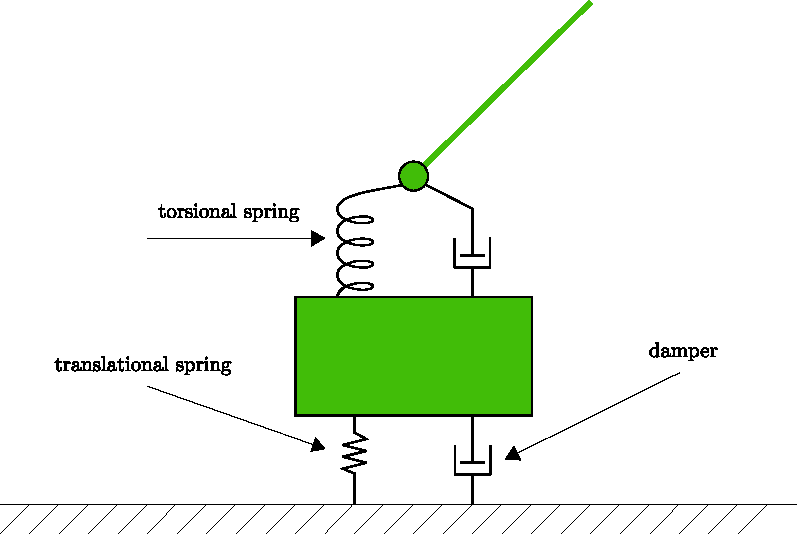
\includegraphics[width=10cm]{Figures/cl_mech_implementation.pdf}
	\caption{Scheme of the system with translational and rotational spring-dampers.}
	\label{fig: cl mechanical implementation}
\end{figure}

These mechanical components provide physical constraints that simplify the learning environment, enabling the agent to gradually adapt to the complex dynamics of the system. As the training progresses, the influence of these spring-damper systems is systematically reduced, allowing the agent to take more control over the system. In the later stages of training, the spring-dampers' effects are diminished, either by reducing their stiffness and damping coefficients or by removing them entirely, thus transferring full control to the learning agent. This transition is crucial for ensuring that the agent is not overly reliant on the physical constraints and is capable of managing the system dynamics independently.
Following this physical setup, We have four parameters in our CL-scheme and their roles are explained in the Table~\ref{table: decay types}. 

\begin{table}[h]
	\caption{Decay types and their descriptions}
	\centering
	\begin{tabular}{m{2.4cm}|m{5cm}}
		\toprule
		\textbf{Curriculum Learning Parameters} & \textbf{Description} \\ \midrule
		Control Values & control parameters representing spring-damper values, which influence the restriction of the system behavior\\ \hline 
		Decay Steps & time steps when the transition to another set of Control Values occurs\\ \hline 
		Decay Function & describes the law on how the Control Values will be changed\\ \hline
		Decay Factor & sets the speed of Decay Function\\ 
		\bottomrule
	\end{tabular}
	\label{table: decay types}
\end{table}

Our approach involves predefined decay functions that dictate the rate and pattern of assistance withdrawal, ensuring a smooth transition of control from the spring-damper systems to the agent. The comparison of decay functions behavior, which are used in our study, is showed at the Figure~\ref{fig: decay functions}.

\begin{figure}[ht]
	\centering
	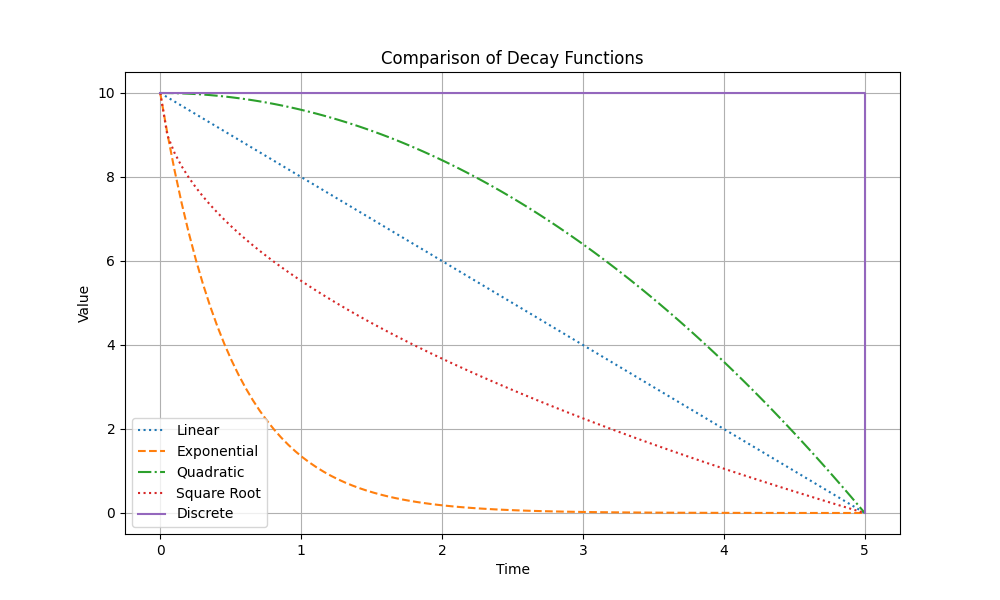
\includegraphics[width=13cm]{Figures/CL_decay_types_comparison.png}
	\caption{5 decay functions comparison for a given set of control values [10, 0]. At the decay step equal to 5 all the functions take the next control value of 0.}
	\label{fig: decay functions}
\end{figure}

In general, decay function could be any function, which will reduce the control values (stiffness and damping coefficients) via some mathematical law.